\section{Research Topics in SSI}

The research focuses on:
\begin{itemize}
    \item the migration of verifiable credentials to post-quantum cryptography (PQC);
    \item the integration of verifiable credentials within the TLS protocol; and
    \item their use within IPsec.
\end{itemize}

\noindent
The latter two are explored in the context of IoT deployments, where credentials are injected directly at lower communication layers to avoid combining traditional certificates and SSI mechanisms.

\subsubsection*{Motivation for Post-Quantum Migration}
Quantum computing is progressing quickly, and the probability that a cryptographically relevant quantum computer becomes available in the future is increasing.\\
Since such systems can efficiently break much of today’s asymmetric cryptography, all identity models relying on standard public-key primitives require a migration strategy. While quantum computing promises major scientific benefits, it simultaneously creates a pressing need to protect Internet protocols and identity mechanisms against quantum adversaries. 
\smallskip

\noindent
The migration to PQC involves two complementary efforts:
\begin{itemize}
    \item \textbf{Definition of PQC algorithms} by cryptographers, based on new hard mathematical problems believed to be resistant to quantum attacks. These schemes are promising but still recent, and their long-term robustness is not yet fully established.
    \item \textbf{Integration of PQC into existing systems and protocols} by engineers. Since protocols and infrastructures cannot be redesigned from scratch, a major challenge is incorporating PQC primitives in a way that preserves compatibility, security, and deployment feasibility.
\end{itemize}

\subsubsection*{Engineering Challenges: Crypto Agility and Deployability}
PQC integration must be performed without disrupting established systems and network operations.

\paragraph*{Crypto Agility}
Crypto agility refers to the ability to reconfigure software and protocols to plug in new cryptographic primitives without extensive refactoring.\\
This requires:
\begin{itemize}
    \item identifying all protocol components relying on cryptography;
    \item refactoring implementations to allow modular replacement of algorithms;
    \item ensuring rapid updates if chosen PQC algorithms are later found vulnerable.
\end{itemize}

\paragraph*{Deployability}
Deployability ensures that PQC-enhanced protocols remain aligned with existing network-management practices:
\begin{itemize}
    \item new mechanisms must support current operational workflows;
    \item no disruptive changes should be introduced for operators and administrators;
    \item standardisation bodies must converge on harmonised integration approaches.
\end{itemize}

\paragraph*{Hybrid Cryptographic Schemes}
During the transition perio are considered. They provide a safety margin: even if a PQC algorithm is later broken, security remains at least as strong as with traditional cryptography. 
\\
Their adoption is still under debate, but they represent a pragmatic approach until pure PQC solutions are fully validated.

\subsubsection*{PQC Algorithms Considered for SSI Migration}
The practical work presented focuses on integrating NIST-selected PQC algorithms into the SSI ecosystem.

\begin{itemize}
    \item \textbf{Key agreement (not directly used in SSI operations):} ML-KEM, HQC.
    \item \textbf{Digital signatures (critical for verifiable credentials):} ML-DSA, SLH-DSA, and Falcon.
\end{itemize}

\noindent
Falcon, although selected by NIST, is less mature for deployment because its floating-point operations introduce potential side-channel vulnerabilities, particularly timing attacks.

\subsubsection*{Use of Verifiable Credentials in TLS and IPsec}
Two research prototypes demonstrate how verifiable credentials can be introduced as certificate types in:
\begin{itemize}
    \item the TLS handshake (layer 4.5), and
    \item IPsec (layer 3).
\end{itemize}

\noindent
The objective is to authenticate endpoints directly within the protocol using verifiable credentials, avoiding the need to first establish secure channels with traditional certificates and then perform higher-layer SSI authentication.\\ 
This is especially relevant for IoT systems, where simplifying identity plumbing across layers can significantly reduce complexity.

%% lezione 21/11

\subsection{Post-Quantum Migration: Performance Evaluation and Algorithm Selection}

Quantum adversaries mainly affect SSI through Shor’s algorithm (impacting discrete logarithms and integer factorisation) and Grover’s search. Since SSI relies exclusively on digital signatures (not on key agreement for encryption) the migration concerns:
\begin{itemize}
    \item post-quantum key-pair generation for issuers and holders;
    \item post-quantum signatures on verifiable credentials (VCs) and verifiable presentations (VPs);
    \item verification of such signatures by verifiers.
\end{itemize}
Only these components require PQC replacement, assuming that the surrounding communication channel (e.g., TLS) is already quantum-resistant.

\subsubsection*{Operational Assumptions}
Two assumptions guide the selection process:
\begin{enumerate}
    \item \textbf{Algorithm selection must consider the signature scheme to be used across issuers, holders, and verifiers.}
    \item \textbf{Verification workloads dominate issuance workloads in web scenarios.}  
    Holders authenticate frequently, whereas credential issuance occurs far less often.  
    Therefore, verifier-side performance is the primary optimisation target.
\end{enumerate}

\subsubsection*{Selection Requirements}
Given the above assumptions and a chosen NIST PQC security level, four requirements were defined (ordered by priority):
\begin{enumerate}
    \item \textbf{Minimal signature verification time}, since the verifier must validate two signatures per authentication (VC and VP).
    \item \textbf{Minimal signature generation time}, to reduce issuer load and minimise the time holders spend preparing VPs.
    \item \textbf{Small signature size}, to limit VC/VP document size and transmission overhead.
    \item \textbf{Small public key size}, beneficial for DID documents or JWK-based identifiers.
\end{enumerate}
Key-pair generation time was not prioritised because keys are generated infrequently in SSI ecosystems.

\subsubsection*{Evaluation of PQC Algorithms}
Using the \texttt{liboqs} library, several signature schemes were benchmarked across the following metrics:
\begin{itemize}
    \item NIST security level;
    \item public key size (JWK-encoded);
    \item signature size;
    \item key-pair generation time;
    \item signature generation time;
    \item signature verification time.
\end{itemize}

\noindent
The comparison included ML-DSA, SLH-DSA (fast and secure variants), and Falcon. Falcon was excluded from the final selection due to incomplete standardisation and susceptibility to timing attacks arising from floating-point operations, despite competitive performance.

\paragraph*{Observed Trends}
Across security levels, the benchmarks revealed that:
\begin{itemize}
    \item public key and signature sizes grow with the security level;
    \item all PQC schemes require significantly more resources than classical algorithms;
    \item ML-DSA consistently offers the best balance of verification time, generation time, and signature size among standardised schemes;
    \item SLH-DSA provides smaller public keys but significantly larger signatures and slower operations;
    \item Falcon shows excellent performance but is unsuitable for deployment today.
\end{itemize}

\subsubsection*{Selection of ML-DSA-44}
Applying the four requirements to empirical results leads to a clear outcome:  
\textbf{ML-DSA-44 (NIST level 2) is the optimal candidate for SSI migration under the stated assumptions.}
\medskip

\noindent
Its verification time, generation time, and signature size outperform other standardised options, particularly in high-frequency verification scenarios.
\smallskip

\noindent
The corresponding security equivalences are:
\begin{itemize}
    \item \textbf{ML-DSA-44 (level 2)}: comparable to SHA-256 collision resistance;
    \item \textbf{ML-DSA-65 (level 3)}: comparable to AES-192 key search;
    \item \textbf{ML-DSA-87 (level 5)}: comparable to AES-256 key search.
\end{itemize}

\subsubsection*{Crypto-Agility as a Design Principle}
The migration does not end with embedding ML-DSA into the SSI framework.\\
To ensure long-term security, the implementation was refactored to support:
\begin{itemize}
    \item modular replacement of signature algorithms;
    \item rapid substitution in case ML-DSA becomes vulnerable;
    \item integration of future PQC candidates without redesigning the framework.
\end{itemize}

\noindent
Crypto agility is therefore not optional but a foundational requirement for PQC adoption in SSI systems.

\subsection *{Hybrid Post-Quantum/Traditional Signatures in SSI}

The migration of SSI toward post-quantum security requires not only crypto agility and deployability but also the adoption of hybrid approaches during the transition.\\
Hybrid schemes combine post-quantum (PQ) and traditional algorithms so that authentication remains secure as long as at least one of the two signature schemes is unbroken. This ensures resilience both against future quantum adversaries and against potential mathematical breakthroughs affecting new PQC primitives.

\subsubsection*{Motivation for Hybridisation}
Although NIST-standardised PQC signatures have undergone rigorous scrutiny, they are still less mature than classical algorithms.\\
A hybrid scheme mitigates this uncertainty: even if a PQC algorithm fails before cryptographically relevant quantum computers emerge, the traditional signature continues to provide security guarantees. Conversely, once such quantum computers become available, PQC components will protect against attacks that break classical signatures.
\medskip

\noindent
The IETF refers to this class of constructions as \textbf{PQ/T hybrid} schemes.

\subsubsection*{Hybrid Signature Scheme}
The hybrid signature is defined as the concatenation of a post-quantum signature and a traditional one:
\[
    \sigma_h = (\sigma_{pq}, \sigma_t).
\]

\noindent
To sign a message \( m \), both algorithms operate on a common modified input:
\[
    m' = \text{hash}(m),
\]
augmented with the DER-encoded object identifier (OID) to prevent cross-protocol substitution.  
\medskip

\noindent
The signing process is:
\[
\begin{aligned}
\sigma_{pq} &\leftarrow \text{Sign}(sk_{pq}, A_{pq}, \text{DER(OID)} \parallel m'), \\
\sigma_{t} &\leftarrow \text{Sign}(sk_{t}, A_{t}, \text{DER(OID)} \parallel m'),
\end{aligned}
\]
where \(A_{pq}\) and \(A_t\) denote algorithm identifiers.

\noindent
Verification requires both signatures to be valid:
\[
\begin{aligned}
\text{Verify}(pk_{pq}, \text{DER(OID)} \parallel m', \sigma_{pq}, A_{pq}), \\
\text{Verify}(pk_{t}, \text{DER(OID)} \parallel m', \sigma_{t}, A_{t}).
\end{aligned}
\]
The hybrid verification succeeds \emph{only if both individual verifications succeed}. An adversary must therefore forge both signatures to impersonate the credential holder.

\subsubsection*{Weak Non-Separability and Stripping Attacks}
A core property of hybrid schemes is \textbf{non-separability}: a verifier must not accept a hybrid signature if one component is missing or stripped.
\medskip

\noindent
Two stripping attack scenarios are possible:
\begin{itemize}
    \item A quantum adversary removes the PQ component and forges the classical signature.
    \item A mathematical break compromises the PQC algorithm, allowing the adversary to remove the classical signature and forge the PQ component.
\end{itemize}

\noindent
Since full non-separability is complex to guarantee in practice, the implemented scheme adopts \textbf{weak non-separability}: an adversary may attempt to remove one component, but \emph{the verifier must detect the stripping}. This is sufficient for transitional security and prevents silent degradation to a broken algorithm.

\subsubsection {Hybridisation Artefact in the DID Document}
To enforce weak non-separability at the protocol level, SSI introduces a \textbf{hybridisation artefact} into the DID Document. This artefact makes explicit the intention of both issuer and holder to use hybrid signatures and ensures that verifiers are aware of the hybrid scheme required for authentication.

\paragraph*{The Composite JWK}
The artefact is encoded as a \texttt{compositeJwk} object extending the JWK format to include:
\begin{itemize}
    \item a post-quantum public key (e.g., ML-DSA-44);
    \item a traditional public key (e.g., Ed25519);
    \item an \texttt{algId} describing the exact hybrid combination.
\end{itemize}

\begin{verbatim}
"compositeJwk": {
  "algId": "id-MLDSA44-Ed25519-SHA512",
  "pqPublicKey": {
     "kty": "ML-DSA",
     "alg": "ML-DSA-44",
     "kid": "...",
     "pub": "... encoded public key ..."
  },
  "traditionalPublicKey": {
     "kty": "OKP",
     "alg": "Ed25519",
     "kid": "...",
     "x": "... encoded coordinate ..."
  }
}
\end{verbatim}

This structure informs the verifier that:
\begin{itemize}
    \item hybrid signatures are mandatory,
    \item both signatures must be checked,
    \item stripping either component invalidates the authentication.
\end{itemize}

\noindent
When verifiable credentials are later anchored to DLTs or quantum-safe ledgers, this artefact will persist as part of the decentralised identity metadata.

\subsubsection*{Security and Deployment Considerations}
The hybrid mechanism supports:
\begin{itemize}
    \item \textbf{crypto agility}: the system can plug in new PQC or classical algorithms as needed;
    \item \textbf{deployability}: no change is required to how operators manage existing systems;
    \item \textbf{transitional robustness}: even if PQC fails early, classical signatures protect authenticity.
\end{itemize}

\noindent
Hybridisation therefore provides a practical and secure pathway from classical SSI to a fully post-quantum identity ecosystem.




\subsubsection *{The \texttt{did:compositejwk} Method and CRUD Operations}

\subsubsection*{Composite JWK in the DID Document}
To support hybrid post-quantum/traditional public keys, the DID Document embeds a
\texttt{compositeJwk} object. The DID is expressed as:
\[
\text{did:compositejwk:}\,\textit{base64url(compositeJwk)}.
\]

\noindent
An example structure is:
\begin{verbatim}
{
  "@context": [
    "https://www.w3.org/ns/did/v1.1",
    "https://w3id.org/security/suites/jws-2020/v1"
  ],
  "id": "did:compositejwk:${base64url-value}",
  "verificationMethod": [{
     "id": "did:compositejwk:${base64url-value}#0",
     "type": "CompositeJsonWebKey",
     "controller": "did:compositejwk:${base64url-value}",
     "compositeJwk": "${composite-jwk}"
  }]
}
\end{verbatim}

\noindent
This design embeds the post-quantum/traditional hybrid key pair directly in the DID method, allowing immediate recovery of the hybrid public keys upon resolution.

\subsubsection*{Definition of the \texttt{did:compositejwk} Method}
The method provides:
\begin{itemize}
    \item a DID mechanism for static PQ/T hybrid keys,
    \item a non-VDR DID method,
    \item an expansion of the encoded composite JWK into a full DID Document.
\end{itemize}

\noindent
Formally:
\[
\text{DID} = \text{did:compositejwk:}\,c\text{-value},
\]
where the \emph{c-value} is a base64url-encoded \texttt{compositeJwk}.

\subsubsection*{CRUD: Create}

\noindent
To create a DID using this method:
\begin{enumerate}
    \item generate or load a \texttt{compositeJwk},
    \item serialize it as a UTF-8 string,
    \item encode the string in base64url,
    \item prefix it with \texttt{did:compositejwk:}.
\end{enumerate}

\noindent
To create the DID Document:
\begin{itemize}
    \item inject the base64url value into the DID,
    \item insert the compositeJwk structure into the verification method.
\end{itemize}

\subsubsection*{CRUD: Resolve}

Resolving a \texttt{did:compositejwk} consists of:
\begin{enumerate}
    \item removing the prefix \texttt{did:compositejwk:},
    \item decoding the remaining string from base64url,
    \item parsing the decoded value as UTF-8 JSON,
    \item validating \texttt{compositeJwk} properties,
    \item generating the DID Document using the hybrid public key.
\end{enumerate}

\noindent
The validation step ensures that both the PQ and traditional public keys conform to the algorithm identifier defined in the composite object.

\subsubsection*{CRUD: Update}

This DID method does not support updates, since the keys are static and directly encoded in the DID itself.

\subsubsection*{CRUD: Deactivate}

This DID method does not support deactivation of the DID Document.


\subsubsection*{Performance Impact}

The DID Document size grows with:
\begin{itemize}
    \item the size of post-quantum public keys,
    \item the security level of ML-DSA variants,
    \item the hybridisation overhead when combining ML-DSA with Ed25519.
\end{itemize}

\noindent
Experimental evaluation confirms:
\begin{itemize}
    \item DID creation time correlates with key pair generation time,
    \item JWT(VC) and JWT(VP) sizes follow the size of PQ signatures,
    \item verification time remains coherent with the timing of the underlying signature algorithms.
\end{itemize}

\subsubsection*{Selection of Algorithms for PQ/T Hybrid VCs and VPs}

The same principles used for pure post-quantum selection apply to hybrid schemes.\\
The chosen combinations are:
\begin{itemize}
    \item \texttt{id-MLDSA44-Ed25519-SHA512},
    \item \texttt{id-MLDSA65-Ed25519-SHA512}.
\end{itemize}

\noindent
These were selected by applying the prioritised criteria: verification time, signature generation time, signature size, and public key size.


\subsection{VC-based TLS handshake for IoT}

Two research works investigate the use of verifiable credentials as alternative certificate types in protocols operating below the application layer of the TCP/IP stack.\\  
The considered protocols are:
\begin{itemize}
    \item TLS,
    \item IPsec.
\end{itemize}

\noindent
Both works assume an \textbf{IoT connected system} as the target scenario.\\ 
The proposed solutions are specifically designed for IoT environments and are not intended to be applied to general-purpose use cases.


\subsubsection*{Research Motivation}

\noindent
Given the advantages in terms of lifecycle management and operational cost reduction, using SSI, the main research question is:

\begin{quote}
Can verifiable credentials be used within TLS to eliminate the need for X.509 certificates?
\end{quote}

\noindent
The motivation is to avoid reliance on traditional identity technologies at the transport layer.\\  
In current architectures, even when SSI is used at the application layer, a TLS channel secured with X.509 certificates is still required.\\ 
The goal is to enable SSI-based authentication directly within TLS.

\subsubsection*{Objectives}

\noindent
The objectives of the proposed solution are:
\begin{itemize}
    \item Extend the TLS~1.3 handshake protocol (RFC~8446) to allow a server, and optionally a client, to authenticate using verifiable credentials.
    \item Preserve interoperability with X.509 public key certificates by supporting:
    \begin{itemize}
        \item hybrid handshakes combining X.509 certificates and VCs,
        \item fallback to the standard TLS~1.3 handshake when necessary.
    \end{itemize}
    \item Preserve all security guarantees provided by the TLS~1.3 handshake, ensuring that confidentiality, integrity, and authentication properties are not weakened.
\end{itemize}

\newpage

\subsection *{VC-based TLS 1.3 Handshake}

\begin{figure}[h]
    \centering
    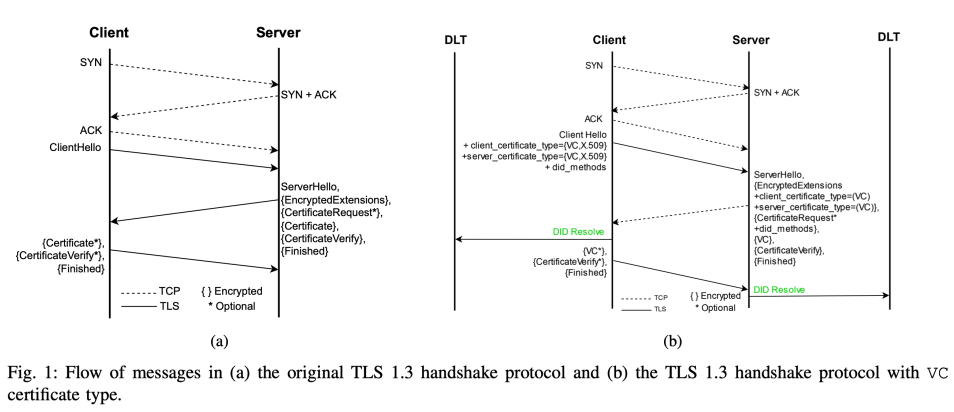
\includegraphics[width=\textwidth]{./images/section_8/comparison_TLS_VCTLS}
    \caption{Comparison between the standard TLS~1.3 handshake and the VC-based TLS~1.3 handshake, highlighting the DID resolution step.}
\end{figure}

\noindent
The TLS~1.3 handshake is extended to support \emph{verifiable credentials (VCs)} as an additional certificate type, while preserving the original protocol structure and security properties.\\ 
The design goal is to minimise protocol changes and ensure full interoperability with existing TLS deployments.

\subsubsection*{Design Principles}

\noindent
The extension of TLS~1.3 follows these principles:
\begin{itemize}
    \item no new handshake messages are introduced,
    \item no existing messages are removed or modified,
    \item only TLS extensions are employed,
    \item backward compatibility with X.509-based authentication is preserved.
\end{itemize}

\noindent
This approach follows the same rationale adopted in RFC~7250, which introduced \emph{raw public keys} as an alternative certificate type to X.509.

\subsubsection {Certificate Type Negotiation}

\noindent
TLS already supports certificate type negotiation through two extensions defined in RFC~7250:
\begin{itemize}
    \item \texttt{client\_certificate\_type},
    \item \texttt{server\_certificate\_type}.
\end{itemize}

\noindent
Originally, these extensions enabled the use of raw public keys in addition to X.509 certificates.\\  
The same mechanism is reused to add \emph{verifiable credentials} as a new certificate type, without altering the semantics of the protocol.

\paragraph{Client Certificate Type}
\noindent
\begin{itemize}
    \item In the \texttt{ClientHello}, it indicates the certificate types the client is able to provide.
    \item In the \texttt{ServerHello}, it indicates the certificate type requested by the server from the client.
\end{itemize}

\paragraph{Server Certificate Type}
\noindent
\begin{itemize}
    \item In the \texttt{ClientHello}, it indicates the certificate types the client is able to process when sent by the server.
    \item In the \texttt{ServerHello}, it indicates the certificate type selected by the server and carried in the \texttt{Certificate} message.
\end{itemize}

\noindent
In all cases, the final decision on the certificate type is taken by the server, as defined by the TLS protocol.

\subsubsection*{DID Method Extension}

\noindent
In addition to the existing certificate type extensions, a new extension called \texttt{did\_methods} is introduced.

\noindent
This extension specifies the DID methods supported by a TLS endpoint and therefore:
\begin{itemize}
    \item the Verifiable Data Registries (VDRs) it can interact with,
    \item where the peer’s DID Document can be resolved.
\end{itemize}

\noindent
The extension follows the standard TLS extension syntax defined in RFC~8446 and contains an enumerated list of supported DID method identifiers. \\ 
Not all endpoints are required to support all DID methods.
\medskip 

\noindent
This mechanism enables interoperability between endpoints using different VDRs, in compliance with the general SSI model.\\
For standardisation purposes, DID method identifiers should be maintained by IANA, similarly to other protocol registries.

\subsubsection*{VC-based Mutual Authentication Flow}

\noindent
The handshake message sequence remains identical to the standard TLS~1.3 handshake.\\ 
The only difference concerns the authentication material exchanged.
\medskip

\noindent
When both client and server support verifiable credentials:
\begin{itemize}
    \item the \texttt{ClientHello} includes:
    \begin{itemize}
        \item \texttt{client\_certificate\_type = \{VC, X.509\}}
        \item \texttt{server\_certificate\_type = \{VC, X.509\}}
        \item \texttt{did\_methods}
    \end{itemize}
    \item the server selects VC as the certificate type,
    \item the \texttt{Certificate} message carries the verifiable credential
    \item the \texttt{CertificateVerify} message signs all previous handshake messages
    \item the \texttt{Finished} message completes the handshake
\end{itemize}

\noindent
VC verification requires an additional operation compared to X.509:
\begin{itemize}
    \item resolution of the DID Document through the selected VDR
\end{itemize}

\noindent
This resolution is performed:
\begin{itemize}
    \item by the client in server-only authentication,
    \item by both endpoints in mutual authentication.
\end{itemize}

\subsubsection*{Why Verifiable Credentials Instead of Verifiable Presentations}

\noindent
Although the SSI model typically relies on \emph{verifiable presentations (VPs)}, the TLS handshake exchanges only verifiable credentials.

\noindent
This choice is justified by the presence of the \texttt{CertificateVerify} message:
\begin{itemize}
    \item it provides a fresh signature over all previous handshake messages
    \item it binds the VC to the current TLS session
    \item freshness is ensured by ephemeral key material in TLS~1.3
\end{itemize}

\noindent
As a result, the security properties normally guaranteed by a VP are preserved:
\begin{itemize}
    \item proof of possession,
    \item freshness,
    \item session binding.
\end{itemize}

\noindent
Avoiding VPs reduces the number of cryptographic operations and mitigates the performance overhead introduced by DID resolution.

\subsubsection*{Hybrid Handshake and Fallback Mechanism}

\begin{figure}[h]
    \centering
    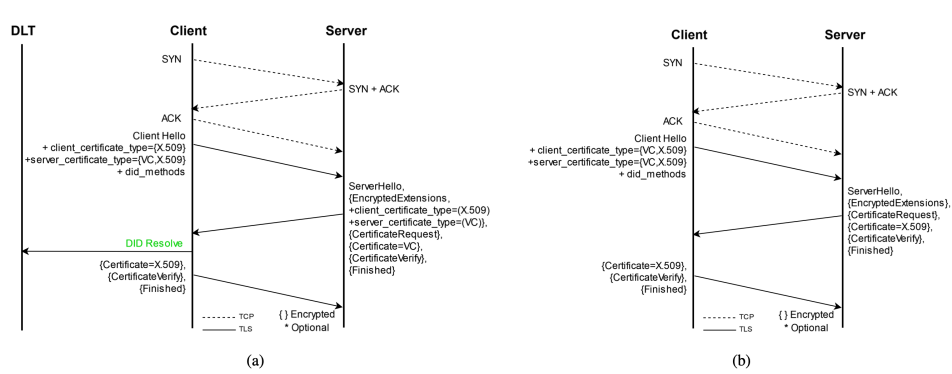
\includegraphics[width=\textwidth]{./images/section_8/hybrid_handshake}
    \caption{Hybrid TLS~1.3 handshake using X.509 and VC certificate types, and fallback to the standard TLS~1.3 handshake.}
\end{figure}

\noindent
Hybrid handshakes are supported, where one endpoint authenticates using X.509 certificates and the other using verifiable credentials\\
For example:
\begin{itemize}
    \item the client authenticates with X.509,
    \item the server authenticates with a VC.
\end{itemize}

\noindent
The VC verification includes DID resolution and revocation status checking, while the X.509 side follows the standard TLS verification process.
\medskip

\noindent
If an endpoint does not support or does not accept VC-based authentication:
\begin{itemize}
    \item certificate type extensions may be ignored,
    \item the handshake falls back to standard X.509-based TLS~1.3.
\end{itemize}

\noindent
This fallback is automatically enabled by reusing existing TLS extensions and guarantees backward compatibility without introducing additional protocol logic.

\subsubsection{Experimental Evaluation}

\noindent
The proposed VC-based TLS~1.3 handshake was implemented in OpenSSL and experimentally evaluated on a real testbed.

\subsubsection*{ Setup}

\noindent
The experimental setup consists of:
\begin{itemize}
    \item two Raspberry Pi devices acting as TLS client and server,
    \item a patched OpenSSL implementation supporting VC-based authentication,
    \item a DLT node used as Verifiable Data Registry (VDR).
\end{itemize}

\noindent
Both Raspberry Pi devices interact with the same DLT node.  
Experiments were conducted considering:
\begin{itemize}
    \item unilateral authentication (server-only),
    \item mutual authentication (client and server).
\end{itemize}

\subsubsection*{Handshake Latency and DID Resolution}

\noindent
Table~\ref{tab:tls_latency} reports the average latency of the overall TLS handshake and the DID resolution phase under different configurations.

\begin{table}[h]
\centering
\caption{Average latency of TLS handshakes and DID resolution in unilateral (UNI) and mutual (MUT) authentication scenarios [ms].}
\label{tab:tls_latency}
\begin{tabular}{l|l|c|c|c}
\hline
 &  & X.509 & HTTP over TCP & HTTP over TCP with IPsec \\ \hline
\multirow{2}{*}{UNI} 
& Handshake & 13.9 & 25.5 & 26.4 \\
& DID resolution & -- & 8.2 & 9.2 \\ \hline
\multirow{2}{*}{MUT} 
& Handshake & 21.0 & 46.4 & 50.0 \\
& DID resolution & -- & 17.8 & 21.4 \\ \hline
\end{tabular}
\end{table}

\noindent
When using verifiable credentials, the additional latency is mainly due to the DID resolution process.\\  
Compared to X.509-based authentication, VC-based handshakes require online interaction with the VDR, whereas certificate chain validation in PKI can be performed offline.
\medskip

\noindent
Securing the communication with the DLT node using IPsec introduces a negligible overhead (approximately 1~ms) compared to unsecured HTTP, while providing strong protection against active attacks.

\subsubsection*{Hybrid Handshake Performance}

\noindent
Table~\ref{tab:hybrid_latency} reports the average latency for hybrid handshakes, where one endpoint uses X.509 and the other uses verifiable credentials.

\begin{table}[h]
\centering
\caption{Average latency of hybrid TLS~1.3 handshakes with IPsec-secured DLT communication [ms].}
\label{tab:hybrid_latency}
\begin{tabular}{c|c|c}
\hline
Server & Client & Handshake latency \\ \hline
X.509 & VC & 41.6 \\
VC & X.509 & 40.7 \\ \hline
\end{tabular}
\end{table}

\noindent
The results show that hybrid handshakes introduce a moderate overhead compared to pure X.509 authentication, while remaining compatible with existing TLS deployments.

\subsubsection*{Security Considerations}

\noindent
A critical security aspect concerns the communication between TLS endpoints and the VDR during DID resolution.
\medskip

\noindent
If the DID resolution process is not protected, an attacker could perform a man-in-the-middle attack by providing a forged DID Document containing a malicious public key.\\  
Since the attacker would control the corresponding private key, the security of the TLS handshake would be compromised.
\medskip

\noindent
To mitigate this risk, three approaches were evaluated:
\begin{itemize}
    \item unsecured HTTP communication with the DLT node
    \item HTTPS communication secured with TLS
    \item IPsec tunnels between TLS endpoints and the DLT node
\end{itemize}

\noindent
Among these options, IPsec provides the best trade-off between security and performance.
\medskip

\noindent
IPsec tunnels can be established once (using IKE) and reused for subsequent DID resolutions, avoiding the overhead of repeatedly establishing TLS connections.\\ 
Key rotation and rekeying are handled automatically by the protocol.
\medskip

\noindent
To avoid reintroducing certificate management overhead, IPsec authentication is performed using \emph{raw public keys} instead of X.509 certificates.
\medskip

\noindent
In a realistic IoT deployment:
\begin{itemize}
    \item many IoT nodes interact with a small number of DLT nodes
    \item each IoT node stores only the public keys of the DLT nodes
    \item DLT nodes maintain a list of trusted IoT public keys
\end{itemize}

\noindent
This model significantly reduces identity management complexity and storage requirements.

\subsubsection*{Privacy Considerations}

\noindent
Two main privacy aspects are considered.

\paragraph{DID Method Disclosure}
\noindent
The \texttt{did\_methods} extension is sent in cleartext within the \texttt{ClientHello}.\\  
This reveals which DID methods are supported by the client.
\smallskip

\noindent
This information is not considered sensitive and does not introduceise significant privacy risks.

\paragraph{DID Resolution Observability}
\noindent
Resolving a server DID on a public DLT allows the DLT node to observe which services a client accesses, similarly to DNS resolution.

\noindent
In IoT scenarios, this is generally not a concern because:
\begin{itemize}
    \item deployments typically operate in a closed and managed environment,
    \item administrators can deploy and control their own DLT entry nodes,
    \item privacy risks are therefore limited to the system owner.
\end{itemize}

\vspace{1.5 cm}

\subsubsection*{Fallback Validation}

\noindent
Fallback to the standard TLS~1.3 handshake was experimentally validated using:
\begin{itemize}
    \item a patched OpenSSL implementation
    \item a vanilla OpenSSL implementation
\end{itemize}

\noindent
When certificate type extensions are not recognised, the handshake successfully falls back to X.509-based authentication, confirming backward compatibility.

\subsubsection*{Discussion and Conclusion}

\noindent
The experimental results show that VC-based TLS authentication introduces a moderate performance overhead due to online DID resolution.

\noindent
However, this overhead does not change the order of magnitude of handshake latency and is largely offset by:
\begin{itemize}
    \item reduced identity lifecycle management costs
    \item simplified key rotation
    \item integrated revocation checking
    \item improved automation in large-scale IoT deployments
\end{itemize}

\noindent
For IoT scenarios where identity management cost is a dominant concern, the use of verifiable credentials in TLS represents a viable and effective alternative to traditional X.509-based PKI.



\subsection{IPsec with Verifiable Credential Certificate Type}

\noindent
Another research work investigates the use of verifiable credentials within IPsec, focusing in particular on the \emph{Internet Key Exchange version~2 (IKEv2)} protocol.
\medskip

\noindent
The motivation is aligned with real-world telco deployments, where IPsec is widely used to establish secure tunnels between network functions (e.g., Kubernetes endpoints) in Software-Defined Networking (SDN) environments.\\  
In such scenarios, identity management based on X.509 certificates introduces significant operational costs.

\subsubsection*{Motivation}

\noindent
Current IPsec deployments rely on centralized PKI and X.509 certificates for endpoint authentication.\\
This results in:
\begin{itemize}
    \item high certificate lifecycle management costs,
    \item significant human intervention,
    \item scalability limitations.
\end{itemize}

\noindent
In practice, some telco operators avoid IKEv2 entirely by adopting centrally controlled IPsec solutions (CCIPS), where keys or key references are distributed directly to endpoints.
\medskip

\noindent
This observation motivates the research question:

\begin{quote}
Can verifiable credentials be used as an alternative certificate type in IKEv2 to reduce identity management costs while preserving IPsec security guarantees?
\end{quote}

\subsubsection {IKEv2 Architecture Overview}

\noindent
IKEv2 operates between two endpoints, each comprising:
\begin{itemize}
    \item an \emph{IKEv2 engine}, responsible for negotiating Security Associations (SAs),
    \item an \emph{IPsec engine}, which uses the negotiated SAs to establish encrypted tunnels.
\end{itemize}

\noindent
IKEv2 exchanges consist mainly of two phases:
\begin{itemize}
    \item \texttt{IKE\_SA\_INIT}, used to negotiate cryptographic parameters, keys, and nonces,
    \item \texttt{IKE\_AUTH}, used for mutual authentication and SA establishment.
\end{itemize}

\begin{figure}[h]
    \centering
    \includegraphics[width=\textwidth]{./images/section_8/ikev2.png}
    \caption{IKEv2 message exchange for mutual authentication (slide 7).}
\end{figure}

\newpage 
\subsubsection {VC-based IKEv2 Handshake}

\begin{figure}[h]
    \centering
    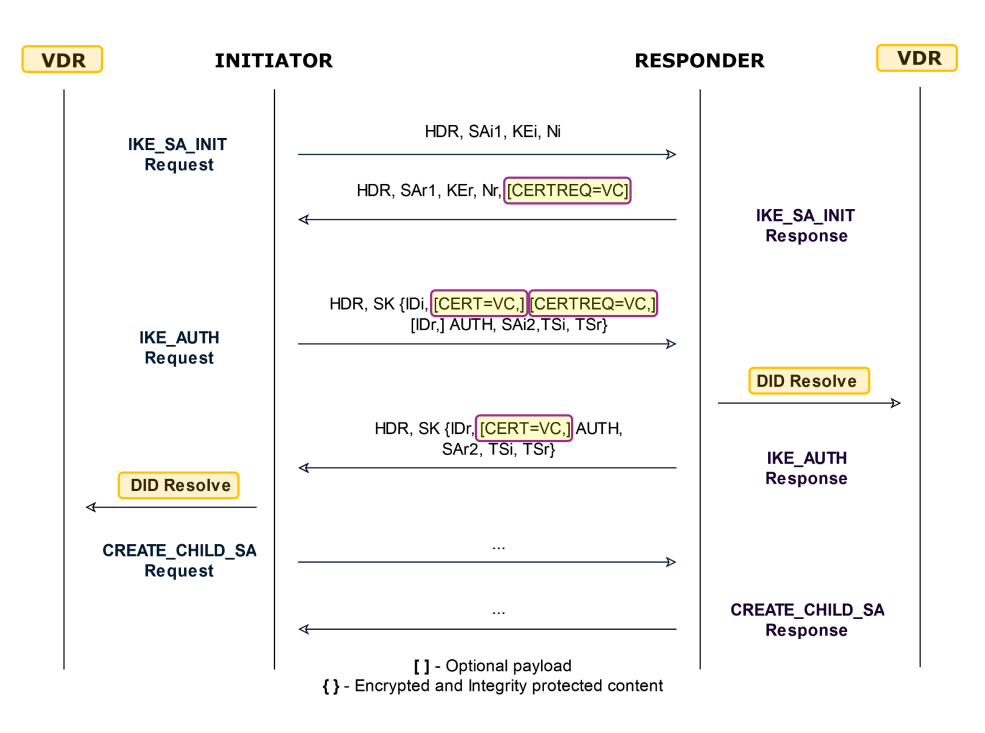
\includegraphics[width=\textwidth]{./images/section_8/ikev2_vc_handshake.png}
    \caption{IKEv2 message exchange extended with Verifiable Credentials and DID resolution (slide 8).}
\end{figure}

\noindent
The proposed solution introduces verifiable credentials as a new \emph{certificate encoding} for IKEv2, without altering the core protocol logic.
\medskip

\noindent
A new certificate encoding value \texttt{VC} is added. \\
When \texttt{VC} is selected:
\begin{itemize}
    \item the \texttt{CERT} payload carries the verifiable credential,
    \item the \texttt{CERTREQ} payload is used to negotiate supported DID methods.
\end{itemize}

\noindent
Specifically, the \emph{Certification Authority} field of \texttt{CERTREQ} contains the list of DID methods supported by the sender, indicating which Verifiable Data Registries (VDRs) can be used to resolve the peer’s DID.

\noindent
As in the TLS-based solution, VC verification requires resolving the DID Document from the VDR.  
Since IKEv2 typically enforces mutual authentication, two DID resolutions are required.

\subsubsection*{Security Considerations}

\noindent
The design does not modify any pre-existing operating principle of the IKEv2 protocol.
\medskip

\noindent
However, if DID resolution is performed over an unsecured channel, a man-in-the-middle attacker could:
\begin{itemize}
    \item impersonate the VDR node,
    \item forge a DID Document binding the peer’s DID to an attacker-controlled key pair,
    \item compute a valid signature in the \texttt{AUTH} payload.
\end{itemize}

\noindent
This would allow the attacker to authenticate successfully using a reused VC.
\medskip

\noindent
To mitigate this threat, the recommended solution is to establish a pre-existing IPsec tunnel with the VDR node hosted and operated by the telco operator.
\medskip

\noindent
Authentication of this tunnel is performed using \emph{raw public keys}, avoiding the reintroduction of X.509 certificate management overhead.

\subsubsection*{Experimental Validation}

\noindent
The solution was experimentally validated on a real testbed.  
Table~\ref{tab:ikev2_latency} reports the average latency of IKEv2 exchanges.

\begin{table}[h]
\centering
\caption{Average latency of IKEv2 exchanges [ms].}
\label{tab:ikev2_latency}
\begin{tabular}{l|c|c}
\hline
 & X.509 & VC \\ \hline
Total latency & 36.7 & 72.6 \\ \hline
Initiator construct CERT & 0.33 & 0.22 \\
Responder construct CERT & 0.29 & 0.14 \\
Initiator construct AUTH & 4.08 & 3.78 \\
Responder construct AUTH & 1.70 & 3.51 \\
Process peer CERT (Initiator) & 0.49 & 18.91 \\
Process peer CERT (Responder) & 0.54 & 21.09 \\
Process peer AUTH (Initiator) & 4.86 & 2.32 \\
Process peer AUTH (Responder) & 3.06 & 3.49 \\ \hline
\end{tabular}
\end{table}

\noindent
The increased latency when using verifiable credentials is almost entirely due to DID resolution.  
Signature generation and verification costs remain comparable, as the same cryptographic algorithms are used.

\subsubsection*{Discussion}

\noindent
While VC-based authentication roughly doubles the IKEv2 setup time, this overhead is negligible in typical IPsec deployments.
\medskip

\noindent
Unlike TLS, where connections are short-lived and handshake latency is critical, IPsec tunnels are usually established once and maintained for long periods (hours or days).
\medskip

\noindent
In this context, an additional delay of a few tens of milliseconds is insignificant, while the reduction in identity management cost is substantial.

\subsubsection*{Conclusion}

\noindent
The use of verifiable credentials in IKEv2:
\begin{itemize}
    \item significantly reduces the cost of identity management for IPsec endpoints,
    \item preserves all security properties of the IKEv2 protocol,
    \item represents a viable solution for real-world telco deployments.
\end{itemize}

\noindent
The same performance trade-offs observed in the TLS-based solution apply here, but their impact is strongly dependent on the operational context, making VC-based IPsec particularly attractive for long-lived secure tunnels.
